% Standalone system-overview figure for the Picbreeder-VLM blog post.
% Compile with: pdflatex system_overview.tex
% Featured agent: agent_781 from th2_ag20_gemini-3-pro-preview_..._s4,
% which branched from the pale "Digital Canary" (img_000685) and published the
% vividly yellow "Yellow Duck Portrait" (img_000783) -- the session where the
% yellow first emerges, so the branched parent looks distinct from the result.
%
% Layout: a true 2x2 grid of equal-sized framed panels (7.7 x 7.7 cm each),
% gap = 2.3 cm horizontally and 0.8 cm vertically. Bitmaps inside the top
% panels are centered (Sampling has some intentional vertical whitespace
% because its native aspect is wider than square).
\documentclass[border=8pt, varwidth=false]{standalone}
\usepackage{tikz}
\usetikzlibrary{positioning,shapes.geometric,arrows.meta,calc,fit,backgrounds,fadings}
\usepackage{graphicx}
\usepackage{amsmath,amssymb}
\usepackage{xcolor}
\usepackage[T1]{fontenc}

% Star ratings (used in Evaluation panel)
\definecolor{ratingGold}{HTML}{DAA520}
\definecolor{ratingGray}{gray}{0.78}
\def\starOn{\textcolor{ratingGold}{$\bigstar$}}
\def\starOff{\textcolor{ratingGray}{$\bigstar$}}
\newcommand{\stars}[1]{\ifcase#1\relax
  \starOff\starOff\starOff\starOff\starOff\or
  \starOn\starOff\starOff\starOff\starOff\or
  \starOn\starOn\starOff\starOff\starOff\or
  \starOn\starOn\starOn\starOff\starOff\or
  \starOn\starOn\starOn\starOn\starOff\or
  \starOn\starOn\starOn\starOn\starOn\fi}

% Featured-agent metadata (pubTitle, parentTitle, featuredAgent, branching
% row labels, rated-cell titles+ratings) regenerated by
% tools/build_system_fig_assets.py. Fallbacks let the figure build standalone.
\IfFileExists{_featured_meta.tex}{% auto-generated by tools/build_system_fig_assets.py
\def\pubTitle{Yellow Duck Portrait}
\def\parentTitle{Digital Canary}
\def\featuredAgent{agent\_781}
\def\branchingRowLabels{0/{top-rated}, 1/{best-new}, 2/{most-\\branched}, 3/{latest}, 4/{random}}
\def\branchingRows{5}
\def\branchingCols{5}
\def\ratedCells{0/Chrome Swan/5, 1/Chrome Heron/4, 2/Abstract Orca/4, 3/Chromatic Seahorse/3, 4/Minimalist Egg/2, 5/Mechanical Eye/1}
}{%
  \def\pubTitle{Cartoon Canary}\def\parentTitle{Rubber Duck Profile}%
  \def\featuredAgent{agent\_909}%
  \def\branchingRowLabels{0/top-rated,1/best-new,2/most-branched,3/latest,4/random}%
  \def\branchingRows{5}\def\branchingCols{5}%
  \def\ratedCells{0/Liquid Metal Spoon/5,1/Luminous Angel/4,2/Elegant Gaze/4,3/Abyssal Fish/3,4/Galactic Sentry/2,5/Chrome Brontosaurus/1}%
}

% Equal panel dimensions for all four quadrants
\def\panelW{7.7cm}
\def\panelH{7.7cm}
% Bottom row (Evolution/Evaluation): a touch taller than content-hugging so the
% Evolution frame fits the published-image thumbnail under the VLM publication
% node, without leaving much dead space in Evaluation.
\def\panelHb{7.3cm}

\begin{document}
\begin{tikzpicture}[
  >=Stealth,
  font=\footnotesize,
  x=1cm, y=1cm,
  box/.style       = {draw, rounded corners=2pt, align=center,
                      inner sep=4pt, line width=0.6pt, fill=white},
  vlmbox/.style    = {box, fill=blue!5,   draw=blue!55!black},
  mutbox/.style    = {box, fill=green!6,  draw=green!55!black},
  img/.style       = {draw=black!45, line width=0.4pt, inner sep=0, outer sep=0},
  pipe/.style      = {->, line width=0.7pt, draw=black!75},
  loop/.style      = {->, line width=0.7pt, draw=blue!55!black, dashed},
  feed/.style      = {->, line width=0.9pt, draw=orange!75!black},
  rate/.style      = {->, line width=0.9pt, draw=green!50!black},
  frame/.style     = {draw=black!45, line width=0.5pt, rounded corners=4pt,
                      inner sep=10pt},
  colTitle/.style  = {font=\bfseries, anchor=south west},
]

% ===================== TOP-LEFT: ARCHIVE =====================
\node[frame, minimum width=\panelW, minimum height=\panelH, anchor=north west]
  (arch) at (0,0) {
\includegraphics[width=7cm]{archive_grid_small.png}};
\node[colTitle] at (arch.north west) {Archive};

% ===================== TOP-RIGHT: SAMPLING =====================
% Stacked outline behind+left to indicate two independent draws
% (one consumed by the evolver, one by the rater).
\node[frame, minimum width=\panelW, minimum height=\panelH, anchor=north east,
      fill=white]
  (strip-bg) at (17.35,0.35) {};
\node[frame, minimum width=\panelW, minimum height=\panelH, anchor=north east,
      fill=white]
  (strip) at (17.7,0) {};
% Title placed first only to anchor the clear/fade below; redrawn on top after.
\node[colTitle] (samptitle) at (strip.north west) {Sampling};
% Clear the back outline under the title, but keep its rounded top-left corner
% (and a sliver of the top edge) visible to the LEFT of the title: sharp left
% edge at the title's west, then a short (less-smooth) fade returns the line on
% the right just past the title.
\fill[white]
  ([xshift=-1pt, yshift=3pt]samptitle.south west)
  rectangle ([xshift=2pt, yshift=7pt]samptitle.north east);
\fill[white, path fading=east]
  ([xshift=2pt, yshift=3pt]samptitle.south east)
  rectangle ([xshift=16pt, yshift=7pt]samptitle.north east);
\node[colTitle] at (strip.north west) {Sampling};

% Pure 5x5 thumbnail strip; row labels overlaid in LaTeX font below.
\def\stripImgW{5.5cm}      % each cell = 5.5/5 = 1.1cm tall+wide
\def\stripCell{1.1cm}
\node[inner sep=0pt, anchor=east] (strip-img)
  at ([xshift=-0.15cm]strip.east)
  {
\includegraphics[width=\stripImgW]{branching_subsample.png}};
\foreach \ri/\lbl in \branchingRowLabels {%
  \node[anchor=east, align=right, font=\footnotesize] at
    ([xshift=-4pt, yshift={-(\ri+0.5)*\stripCell}]strip-img.north west) {\lbl};
}

% sample arrow at the (frame-)midline
\draw[feed] (arch.east) -- (arch.east -| strip.west);

% ===================== BOTTOM-LEFT: EVOLUTION =====================
% Fixed-position frame; content placed at known coords inside.
\node[frame, minimum width=\panelW, minimum height=\panelHb, anchor=north west]
  (evo) at (0,-8.5) {};
\node[colTitle] at (evo.north west) {Evolution};

% Three nodes (VLM selection / Mutation-crossover / generation grid), vertically
% centred within the frame: column centre at mut-(2.7225-h_box)/2 = frame centre.
\node[mutbox] (mut) at (3.5,-10.0) {Mutation/crossover};
\node[vlmbox, above=0.4cm of mut] (sel) {VLM selection};
\draw[pipe] (sel) -- (mut);

\node[img, below=0.4cm of mut] (pop0)
  {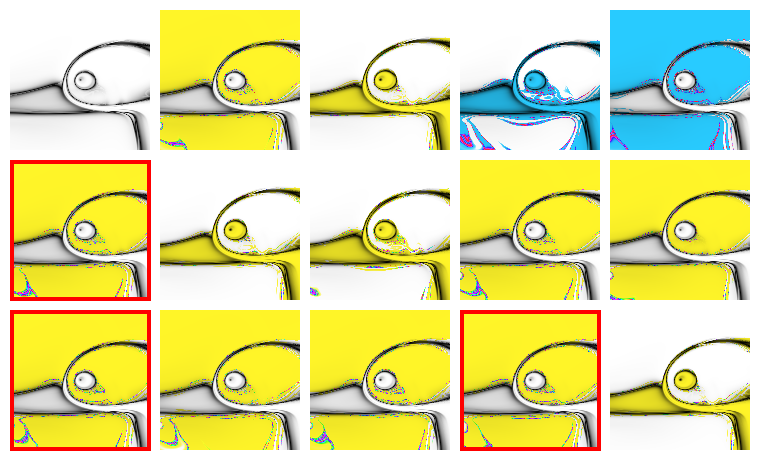
\includegraphics[width=4.5cm]{candidate_grid.png}};
\draw[pipe] (mut) -- (pop0);

% x20 back-edge: leave the generation grid's right edge, sweep up in a symmetric
% curve to the point directly above it (at VLM selection's height), then run as a
% straight horizontal line left into the right side of VLM selection.
\draw[loop]
  (pop0.east) .. controls +(1.4,0) and +(1.4,0) ..
    node[pos=0.5, right=1pt, font=\scriptsize\itshape] {$\times 20$}
    (pop0.east |- sel.east)
  -- (sel.east);

% After the x20 inner loop converges, the agent publishes its favourite back to
% the archive. The publication node sits below the candidate grid, and the actual
% published image is shown beneath it -- that image is what travels to the archive
% (the selection node only feeds the inner loop).
\node[vlmbox, below=0.3cm of pop0] (pub) {VLM publication};
\draw[pipe] (pop0) -- (pub);
\node[img, below=0.24cm of pub] (pubimg)
  {
\includegraphics[width=1.08cm]{publication.png}};
\draw[pipe] (pub) -- (pubimg);

% ===================== BOTTOM-RIGHT: EVALUATION =====================
\node[frame, minimum width=\panelW, minimum height=\panelHb, anchor=north east]
  (eval) at (17.7,-8.5) {};
\node[colTitle] at (eval.north west) {Evaluation};

% Column content: rat-title + 6 rated thumbnails in a 3x2 grid; titles
% and stars are rendered as LaTeX text (not baked into the PNGs).
\node[vlmbox, anchor=north] (rat-title) at (13.85,-8.88) {VLM rating};

\def\rThumb{1.45cm}
\def\rCellW{2.28cm}     % horizontal cell pitch (max that fits in 7cm interior)
\def\rRowGap{1.25cm}    % vertical gap between rows -- clears 2-line title + stars + vspace
\def\rTitleH{0.6cm}     % space reserved below each image for the (up to 2-line) title,
                        % so the stars sit on a fixed baseline and align across a row
\foreach \ic/\ti/\ra in \ratedCells {%
  \pgfmathtruncatemacro{\rr}{\ic / 3}%
  \pgfmathtruncatemacro{\cc}{\ic - 3*\rr}%
  \node[inner sep=0pt, anchor=north] (rt-\ic) at
    ([xshift={(\cc-1)*\rCellW},
      yshift={-0.55cm - \rr*(\rThumb+\rRowGap)}]rat-title.south)
    {\includegraphics[width=\rThumb]{rated_thumb_\ic.png}};
  % Title hangs directly under the image and may wrap to two lines (grows down).
  \node[anchor=north, align=center, inner sep=1pt, text width=\rCellW]
    at ([yshift=-1pt]rt-\ic.south)
    {\hyphenpenalty=10000\exhyphenpenalty=10000\relax
     {\itshape\fontsize{6pt}{7pt}\selectfont\ti}};
  % Stars sit at a fixed drop below the image south -- independent of title length --
  % so every row of stars is vertically aligned.
  \node[anchor=north, inner sep=0pt]
    at ([yshift=-\rTitleH]rt-\ic.south)
    {\scriptsize\stars{\ra}};
}
\node[fit=(rt-0)(rt-1)(rt-2)(rt-3)(rt-4)(rt-5), inner sep=0pt] (rated) {};
\draw[pipe] (rat-title) -- (rt-1.north);

% ===================== CROSS-ARROWS =====================
% Sampling -> VLM selection: leave from the SHADOW frame's west edge, partway down
% (between the incoming sample arrow at the mid-line and the bottom) -- this is the
% evolver's draw, a *different* sample than the one the rater sees. Step LEFT into
% the inter-column whitespace (gap midline = 8.85; strip-bg.west is at x=9.65, so
% step -0.8), drop into the Archive/Evolution gap (mid -8.1), then -| into the top
% of the VLM selection node (clear of the x20 loop). Columns: left=[0,7.7], right=[10,17.7].
\draw[feed]
  ($(strip-bg.west)!0.58!(strip-bg.south west)$)
    -- ++(-0.8,0) -- (8.85,-8.1) -| (sel.north);

% Publish -> archive: the published image leaves its thumbnail on the left,
% routes up *outside* the Evolution frame (clear of its title), and enters
% Archive west BELOW the ratings arrow so the two segments don't cross.
\draw[feed]
  (pubimg.west) -- ([xshift=-0.6cm]evo.west |- pubimg.west)
              |- ([yshift=-0.18cm]arch.west);

% Sampling -> VLM rating: straight vertical, horizontally centered on rater
\draw[feed]
  (strip.south -| rat-title.north) -- (rat-title.north);

% Rater -> archive: leave Evaluation from its bottom center, route under both
% bottom frames and up outside the Evolution frame (further left than the
% Publish arrow), enter Archive west ABOVE the publish arrow.
\draw[rate]
  (eval.south) -- ++(0,-0.5)
                -| ([xshift=-1.0cm, yshift=0.18cm]arch.west)
                -- ([yshift=0.18cm]arch.west);

\end{tikzpicture}
\end{document}
